\subsection{Annotation flow}
\begin{figure}[h]
    \centering
    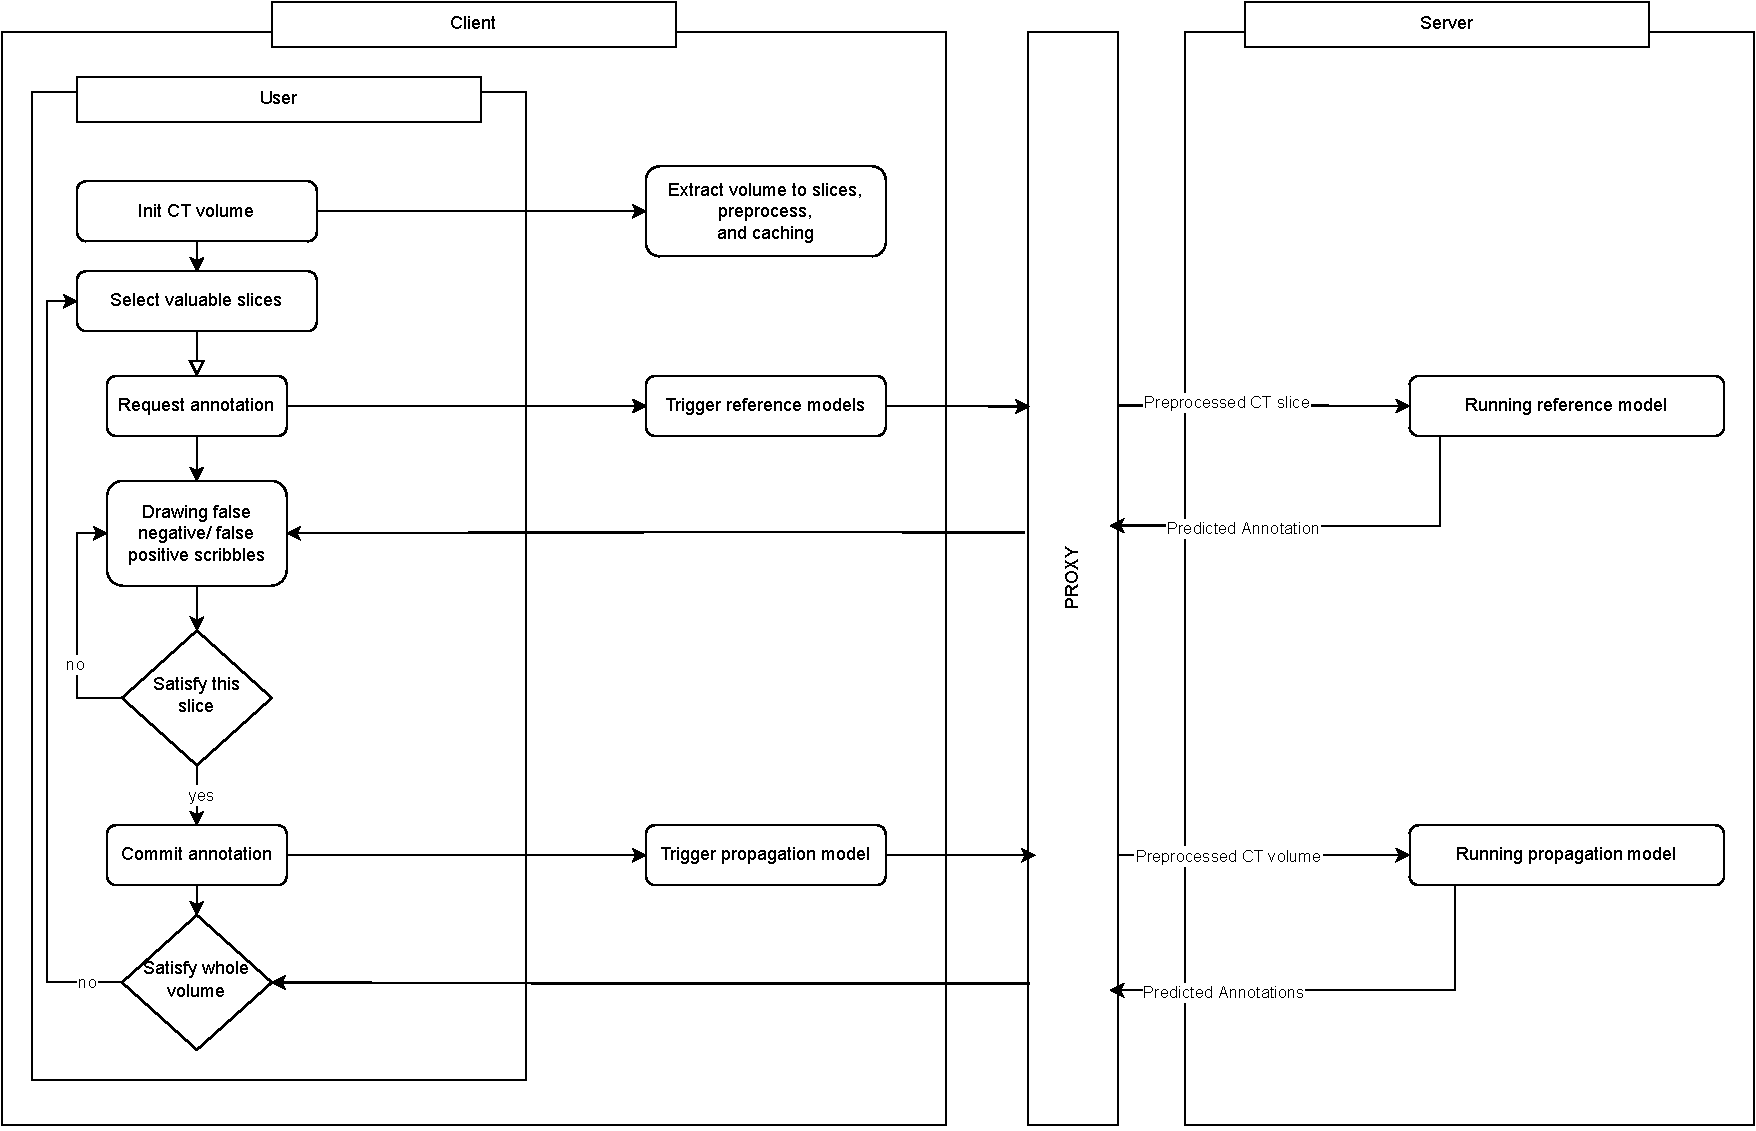
\includegraphics[width=\textwidth]{content/resources/new_images/application/Annotation_flow.pdf}
    \caption{The annotation flow for a CT volume}
    \label{fig:anno_flow}
\end{figure}
The annotation flow in Figure \ref{fig:anno_flow} shown in the diagram illustrates how users, clients, and servers interact with the other. After initialization, the annotator will select valuable slices for the refinement stage. The client will then wrap these slices and send them to the server. The request and response process will be communicated through a proxy. After the server has done its prediction on the whole volume image based on annotations from the refinements made by the annotator, this process will repeat until an acceptable level of results is achieved.

\subsubsection{Request parsing}
The serialization and deserialization processes is very important when it comes to exchanging data between the client and server. By using request parsing, we are able to use JSON for both the client and server messages. This makes the process quick and easy, while also ensuring that all of the data is properly transferred. There are some basic types that can be easily jsonified, such as numbers and strings. However, images and masks need to be encoded using the latin-1 encoder in order to ensure successful transmission.